\documentclass[12pt]{article}

% basic preamble for any kind of document

\usepackage{xcolor}
\usepackage{amsmath}
\usepackage{geometry}
\usepackage{graphicx}
\usepackage{appendix}
\usepackage{setspace} % double spacing
					  % use \doublespacing

\setlength{\parindent}{0pt}

\definecolor{blue}{RGB}{0,114,178}
\newcommand{\fix}[1]{\textcolor{blue}{\textbf{#1}}}

\usepackage{titlesec} % what does this do?


\begin{document}

\subsection*{(a) normalize prices}
We can normalize $\pi_1 = \pi_2 = 1$ without loss of generality because \fix{reason}. 

\subsection*{(b) simulate data}
I simulate data for $N=1000$ observations. See attached Julia code. 

\subsection*{(c) choose true parameters}
After tinkering around, I find parameters $ \theta = ($$1.00$$,\;$$1.00$$,\;$$0.95$$,\;$$0.90$$,\;$$0.20$$,\;$$0.20$$,\;$$0.30$$)$ which results in $57.60$\% of the population choosing occupation 1.

\subsection*{(d) maximum likelihood estimator}
I choose to do maximum likelihood estimation. Define $\Omega$ as the data available to the econometrician, then the likelihood function is 
\begin{align*}
    L(\theta | \Omega ) & = \Pi_{i = 1}^N Pr(w = w_1, d = 1)^d Pr(w = w_0, d = 0)^{1-d}
    \\
    & = \Pi_{i = 1}^N Pr(w = \pi_1 s_1, \pi_1 s_1 > \pi_2 s_2)^d 
                      Pr(w = \pi_2 s_2, \pi_2 s_2 > \pi_1 s_1)^{1-d}
    \\
    & = \Pi_{i = 1}^N Pr(w = \pi_1 e^{\mu_1 + \epsilon_1}, \pi_1 e^{\mu_1 + \epsilon_1} > \pi_2 e^{\mu_2 + \epsilon_2})^d 
                      Pr(w = \pi_2 e^{\mu_2 + \epsilon_2}, \pi_2 e^{\mu_2 + \epsilon_2} > \pi_1 e^{\mu_1 + \epsilon_1})^{1-d}
\end{align*}
I will show the simplification for one of the probabilities, but the steps are pretty much the same for each. We want to ``solve'' for the $\epsilon$'s, since we know their distributions (assuming our assumptions are the truth, that is):
\begin{align*}
    & = Pr(w = \pi_1 e^{\mu_1 + \epsilon_1},\; \pi_1 e^{\mu_1 + \epsilon_1} > \pi_2 e^{\mu_2 + \epsilon_2})
    \\
    & = Pr(\epsilon_1 = \log\big(\frac{w}{\pi_1}\big)-\mu_1,\; 
        \epsilon_2 < \log(\frac{\pi_1}{\pi_2}) +\mu_1 -\mu_2+\epsilon_1 )
    \\
    & = Pr(\epsilon_2 < \log\big(\frac{\pi_1}{\pi_2}\big) +\mu_1 -\mu_2+\epsilon_1 | \epsilon_1 = \log\big(\frac{w}{\pi_1}\big)-\mu_1) \times
        Pr(\epsilon_1 = \log\big(\frac{w}{\pi_1}\big)-\mu_1)
    \\
    & = Pr(\epsilon_2 < \log\big( \frac{w}{\pi_2} \big) - \mu_2 | \epsilon_1 ) 
        \times Pr(\epsilon_1 = \log\big(\frac{w}{\pi_1}\big)-\mu_1)
\end{align*}

since joint distributions can be written as the multiplication of a conditional and a marginal. Note that 
\[ \epsilon_2|\epsilon_1 \sim N \big(\frac{\sigma_{12}}{\sigma_2^2} \epsilon_1,
    \sigma_1^2 - \frac{\sigma_{12}^2}{\sigma_2^2}\big) \]
then the likelihood function becomes 
\[L =  \Pi_{i = 1}^N \bigg[ F_{\epsilon_2 |\epsilon_1} \bigg(\log \big(\frac{w}{\pi_2}\big) - \mu_2\bigg)f_{\epsilon_1} \bigg(\log \big(\frac{w}{\pi_1}\big) - \mu_1 \bigg)\bigg]^d 
\times  
\bigg[ F_{\epsilon_1 |\epsilon_2} \bigg(\log \big(\frac{w}{\pi_1}\big) - \mu_1\bigg) f_{\epsilon_2} \bigg(\log \big(\frac{w}{\pi_2}\big) - \mu_2 \bigg)\bigg]^{1-d}
    \]
And the estimator is 
\[ \hat\theta = argmax_{\theta} \log(L)\]
which is consistent. 


\subsection*{(e) estimate $\mu_1$ and $\rho$ }    
Estimating the parameters with MLE, I find $\hat\mu_1 =$$0.949$ and $\hat\rho =$$0.229$.

\subsection*{(f) identification figures}
\begin{center}
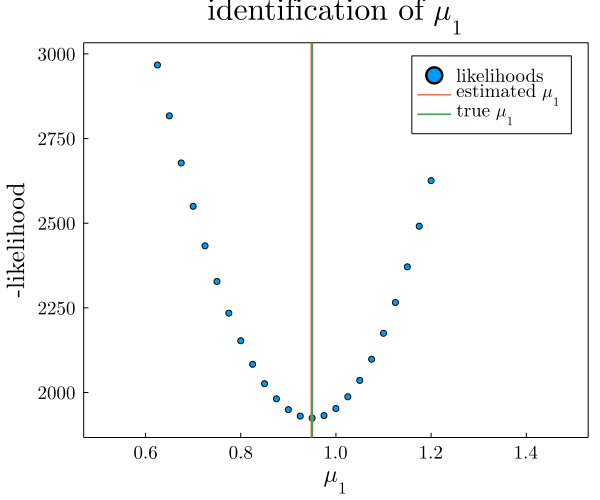
\includegraphics[scale = 0.5]{output/mu_id.png}
\\
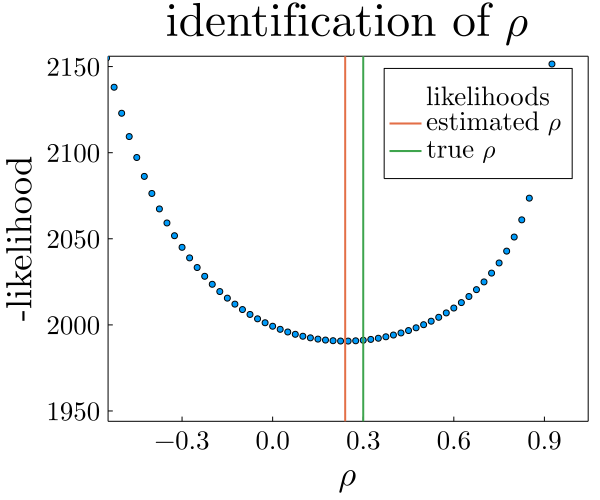
\includegraphics[scale = 0.5]{output/rho_id.png}
\end{center}

\subsection*{(g) compare the data to the model}
\begin{table}[!h]
\centering
 \caption{} \;\begin{tabular}{rrr}
\toprule
 & \textbf{data} & \textbf{model}\\
\midrule
$\mu_1$ & 0.95 & 0.95\\
$\rho$ & 0.30 & 0.23\\
$\textrm{\% in job 1}$ & $60.40$ & 60.30\\
mean $w_1$ & 2.80 & 2.85\\
$\sigma_1$ & 0.46 & 0.53\\
mean $w_2$ & 2.80 & 2.85\\
$\sigma_2$ & 0.46 & 0.53\\
\bottomrule
\end{tabular}
\end{table}

\subsection*{(h) counterfactual}
Suppose that there is a minimum wage of 
$\underline{w_1} =$$2.45$.
The resulting changes are in Table 2, and we see that the average wage for those choosing job 1 is decreasing, though not by much. The average wage for those choosing job 2 increased. This might feel counterintuitive, since we raised the $w_1$ that some individuals might face. However there are some individuals who, before the minimum wage, faced $w_1 < w_2 < \underline{w_1}$, so originally they choose the second job. These were individuals who were pretty low skilled in job 2, and due to correlation, also low waged in job 1, but who are now going to migrate to job 1, bringing the average wage and average skill level down. When low-skilled workers leave job 2, the remaining high-skilled workers bring the average job 2 wage up higher. 
\begin{table}[!h]
\centering
 \caption{} 
\begin{tabular}{rrr}
\toprule
 & \textbf{model} & \textbf{counterfactual}\\
\midrule
\% in job 1 & $56.00$ & 0.67\\
mean $w_1$ & 2.81 & 2.80\\
$\sigma_1$ & 0.49 & 0.42\\
mean $w_2$ & 2.81 & 2.97\\
$\sigma_2$ & 0.49 & 0.38\\
\bottomrule
\end{tabular}
\end{table}


\end{document}